%% LaTeX-Beamer template for KIT design
%% by Erik Burger, Christian Hammer
%% title picture by Klaus Krogmann
%%
%% version 2.1
%%
%% mostly compatible to KIT corporate design v2.0
%% http://intranet.kit.edu/gestaltungsrichtlinien.php
%%
%% Problems, bugs and comments to
%% burger@kit.edu

\documentclass[18pt]{beamer}

%% SLIDE FORMAT

% use 'beamerthemekit' for standard 4:3 ratio
% for widescreen slides (16:9), use 'beamerthemekitwide'

\usepackage{templates/beamerthemekit}
% \usepackage{templates/beamerthemekitwide}

%% TITLE PICTURE

% if a custom picture is to be used on the title page, copy it into the 'logos'
% directory, in the line below, replace 'mypicture' with the 
% filename (without extension) and uncomment the following line
% (picture proportions: 63 : 20 for standard, 169 : 40 for wide
% *.eps format if you use latex+dvips+ps2pdf, 
% *.jpg/*.png/*.pdf if you use pdflatex)
\titleimage{Webinterface_desktop_klein}

%% TITLE LOGO

% for a custom logo on the front page, copy your file into the 'logos'
% directory, insert the filename in the line below and uncomment it

%\titlelogo{Webinterface_desktop_klein}

% (*.eps format if you use latex+dvips+ps2pdf,
% *.jpg/*.png/*.pdf if you use pdflatex)

%% TikZ INTEGRATION

% use these packages for PCM symbols and UML classes
% \usepackage{templates/tikzkit}
% \usepackage{templates/tikzuml}

% the presentation starts here

\title[PCC]{Privacy Crash Cam:\\ Pflichtenheft}
\subtitle{App, Web-Interface und Web-Dienst}
\author{Giorgio G., Christoph H., David L.,  Josh R.,  Fabian W.}

\institute{Karlsruher Institut f\"ur Technologie, Fraunhofer Institut für Optronik, Systemtechnik und Bildauswertung}

% Bibliography

\usepackage[citestyle=authoryear,bibstyle=numeric,hyperref,backend=biber]{biblatex}
\addbibresource{templates/example.bib}
\bibhang1em

\begin{document}

% change the following line to "ngerman" for German style date and logos
\selectlanguage{english}

%title page
\begin{frame}
	\titlepage
\end{frame}

\section{Aufgabenstellung}
\begin{frame}{Aufgabenstellung}
	\begin{itemize}
		\item Verschl\"usselnde Crashcam-App
		\pause
		\item Web-Dienst für Entschl\"usselung, Bildauswertung und Anonymisierung
		\pause
		\item Web-Interface zur Videoverwaltung
	\end{itemize}
\end{frame}

\section{Verschl\"usselnde Crashcam-App}
\begin{frame}{Verschl\"usselnde Crashcam-App}
	\begin{itemize}
		\item 2 Modi
		\pause
		\begin{itemize}
			\item Beobachtungsmodus
			\pause
			\item Aufnahmemodus
		\end{itemize}
		\pause
		\item Men\"u
		\pause
		\begin{itemize}
			\item Kamera
			\pause
			\item Videos
			\pause
			\item Einstellungen
		\end{itemize}
	\end{itemize}
\end{frame}

\section{Web-Interface}
\begin{frame}{Web-Interface}
	\begin{itemize}
		\item Accountverwaltung
		\pause
		\item Ansicht anonymisierter Videos
	\end{itemize}
\end{frame}

\section{Web-Dienst}
\begin{frame}{Web-Dienst}
	\begin{itemize}
		\item Nimmt Anfragen der App und des Web-Interface entgegen
		\pause
		\item Analyse und Anonymisierung der Videos
		\pause
		\item Datenverwaltung
	\end{itemize}
\end{frame}

\section{Organisation}
\begin{frame}[allowframebreaks]{Organisation}
	\begin{figure}
		\begin{center}
			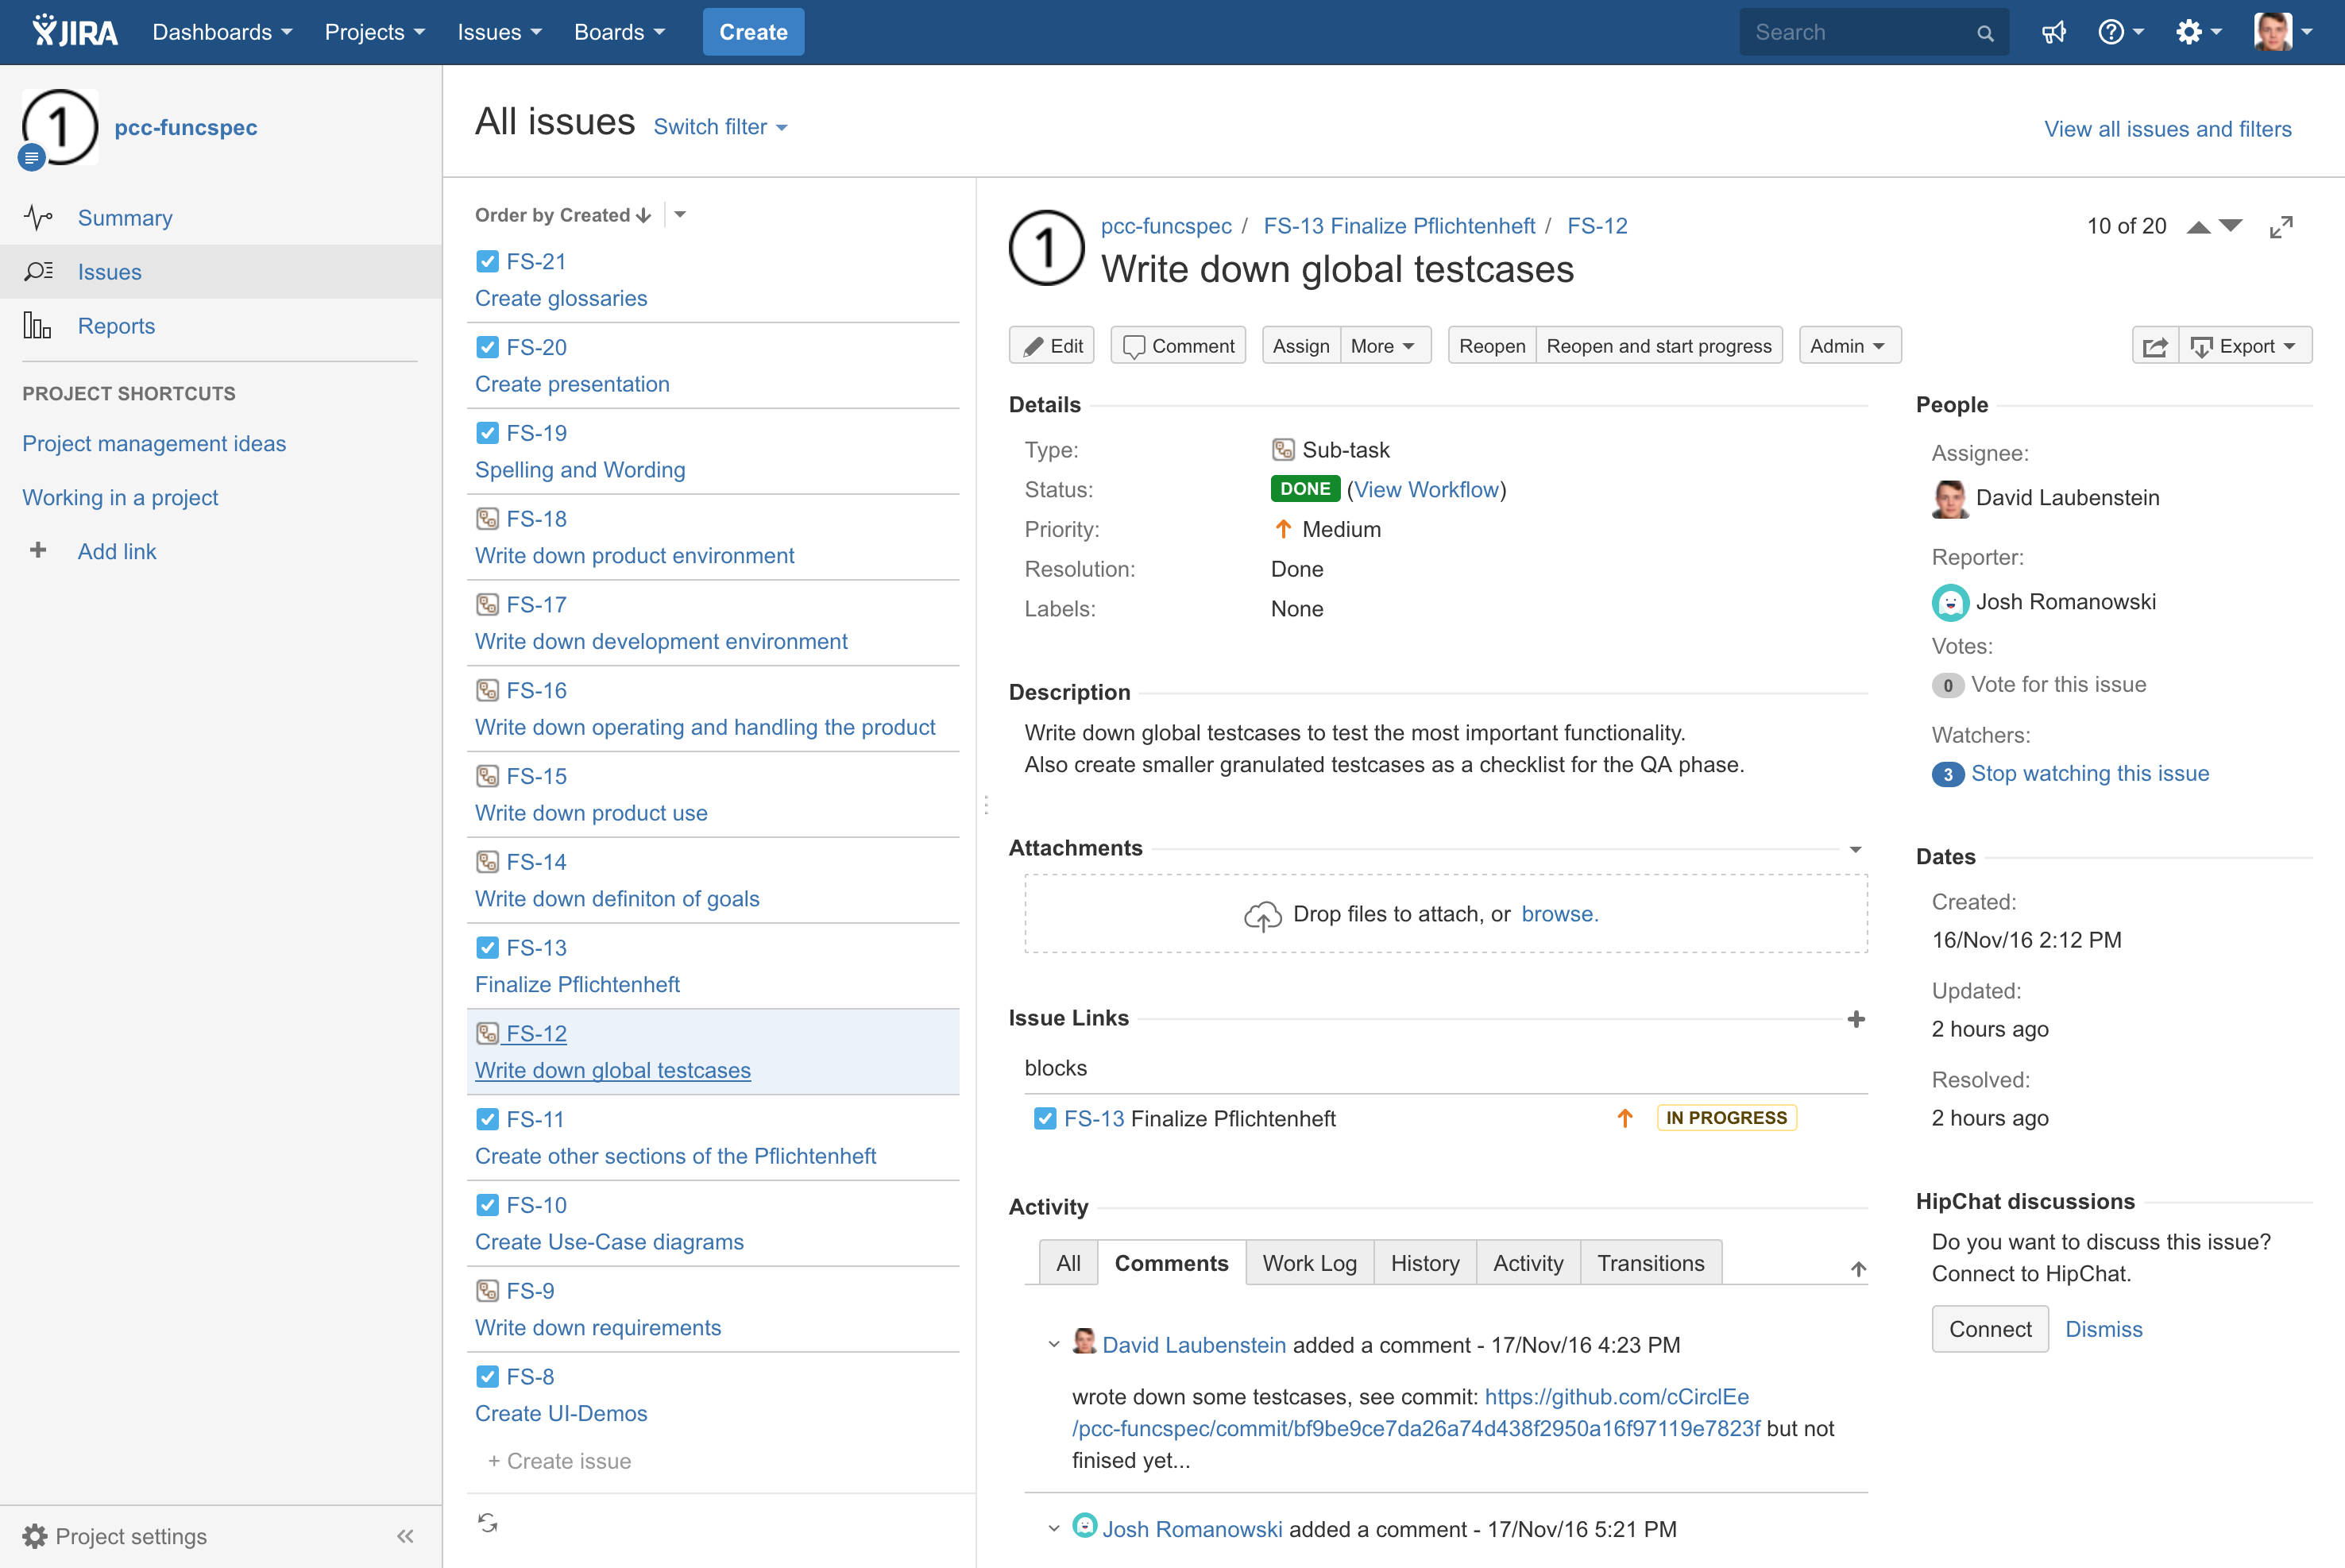
\includegraphics[scale=0.16]{logos/JIRA01} 
		\end{center}
		\caption{Die Abbildung zeigt unser JIRA}
		\framebreak
		\begin{center}
			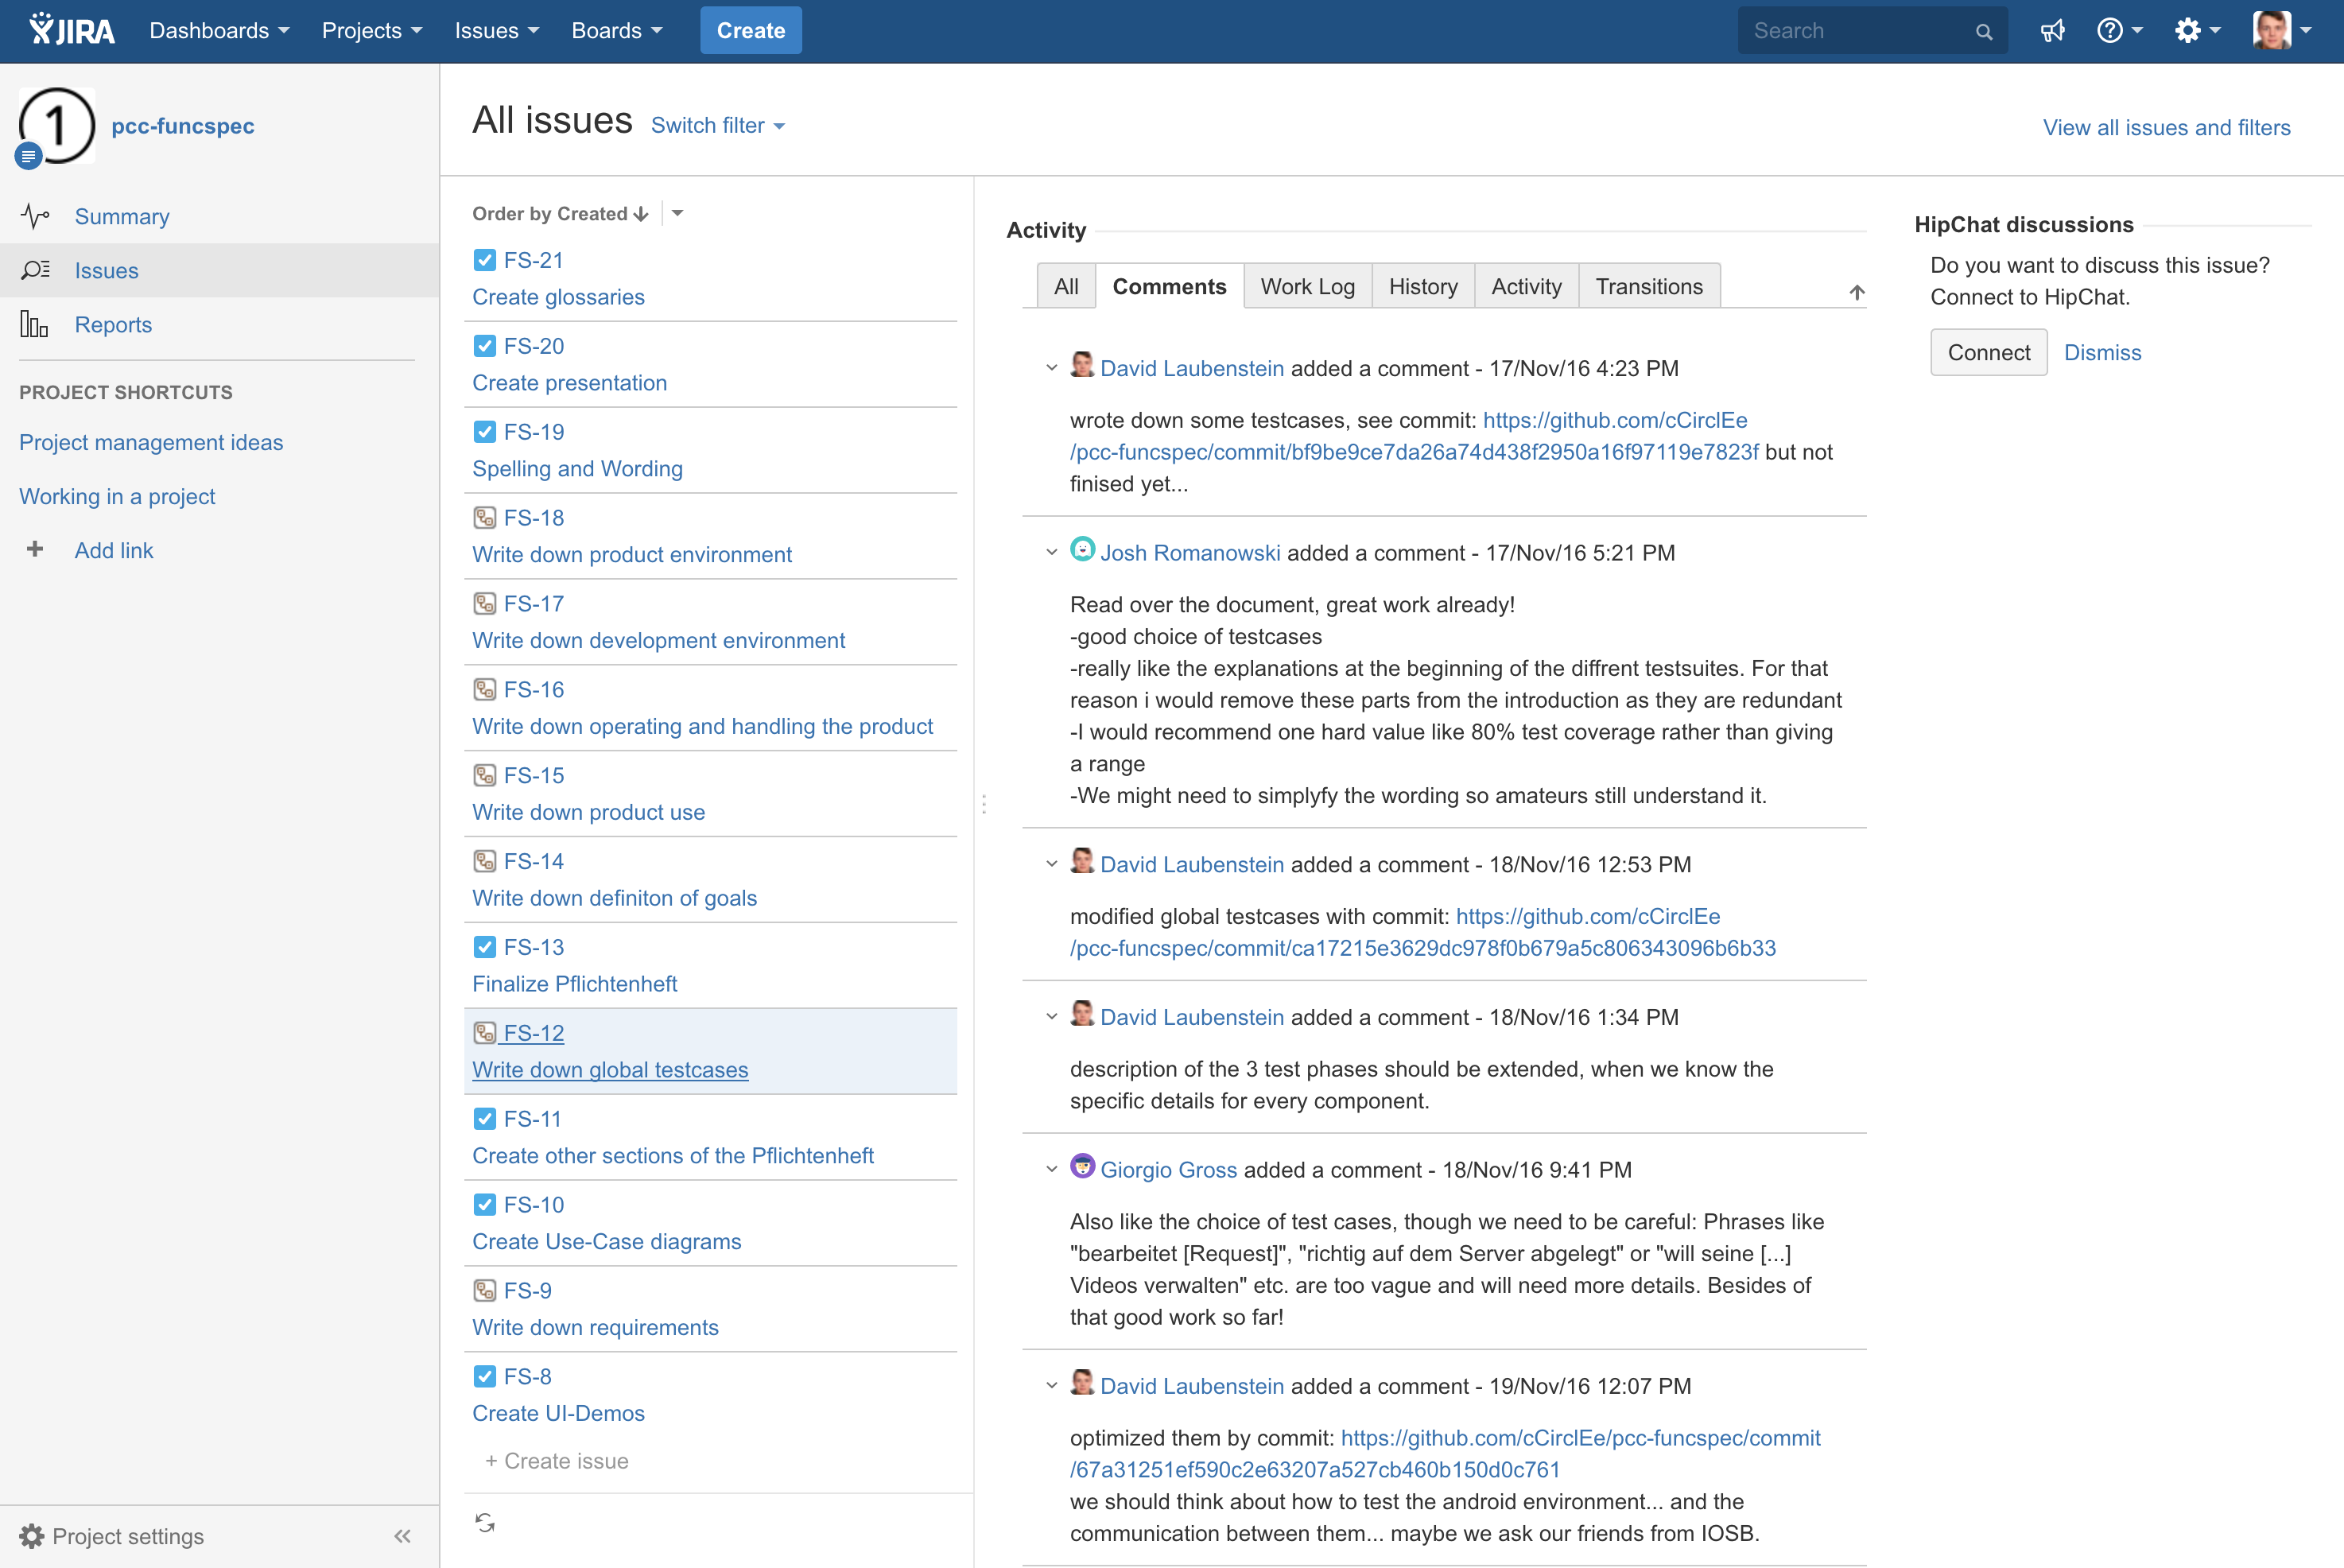
\includegraphics[scale=0.16]{logos/JIRA02} 
		\end{center}
		\caption{Die Abbildung zeigt unser JIRA}
	\end{figure}
	\framebreak
	\begin{figure}
		\begin{center}
			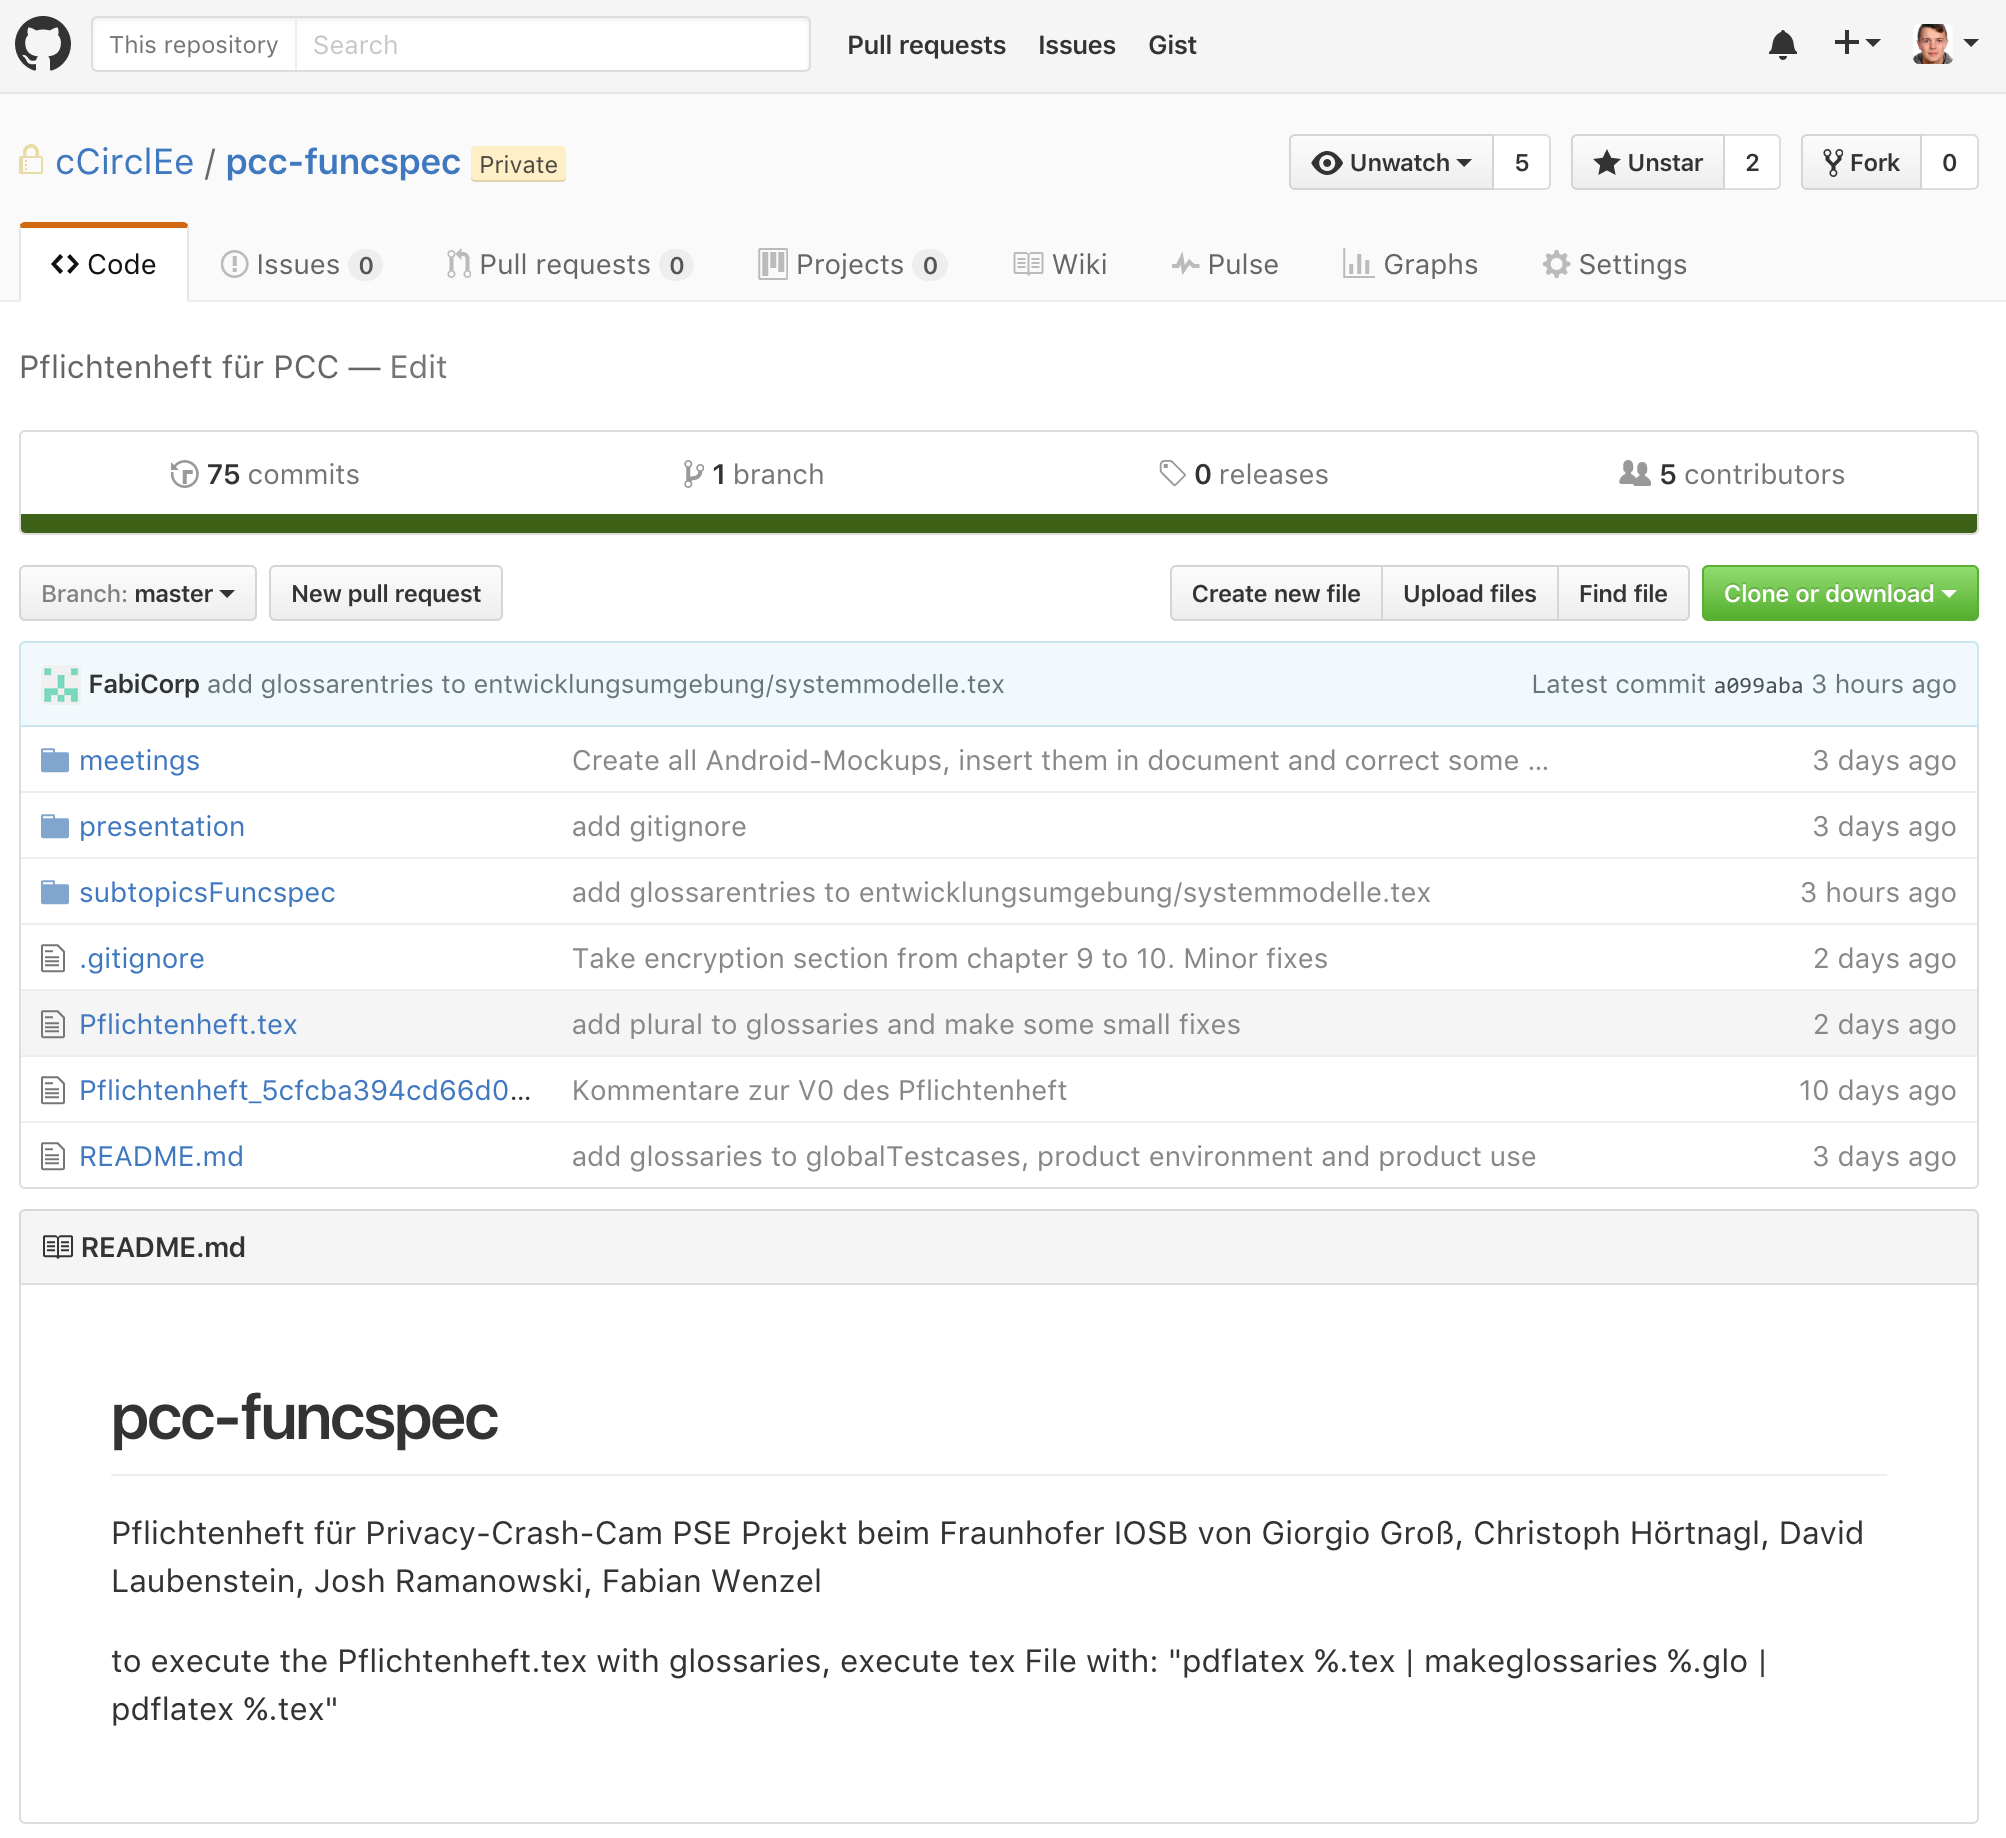
\includegraphics[scale=0.22]{logos/Github} 
		\end{center}
	\end{figure}				
\end{frame}

\section{Gruppenarbeit}
\begin{frame}{Gruppenarbeit}
	\begin{figure}
		\begin{center}
			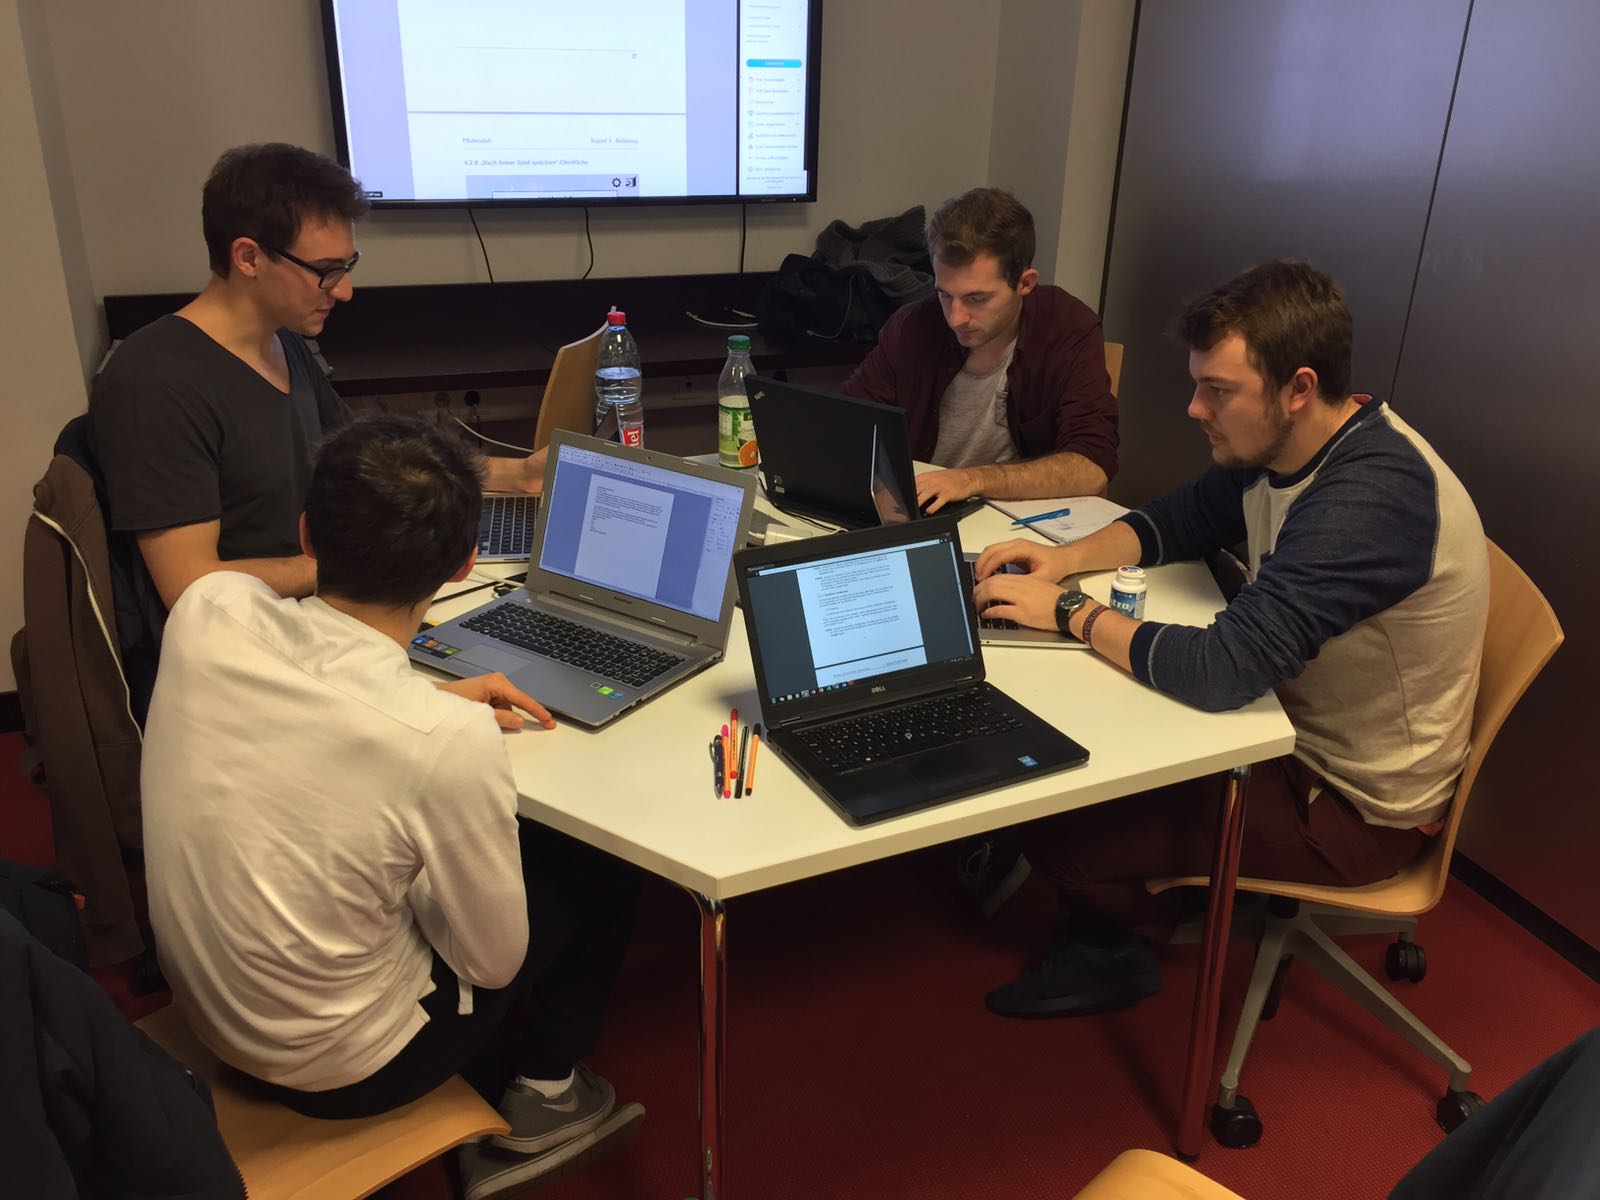
\includegraphics[scale=0.16]{logos/Gruppenarbeit} 
		\end{center}
	\end{figure}		
\end{frame}

\section{}
\begin{frame}
	\begin{center}
 		Vielen Dank f\"ur Ihre Aufmerksamkeit!
	\end	{center} 	
\end{frame}
\end{document}
